\chapter{Desenvolvimento e Testes}
\label{chap:result}



%--------- NEW SECTION ----------------------

\section{Lista de materiais}
No sistema de Percepção os sensores atuam como os sentidos do robô, recebendo dados externos e informando a unidade central de processamento os seus significados. Quanto maior o número de grandezas físicas analisadas, mais complexo o sistema de Percepção e maior a sua capacidade de compreensão.

Os sensores que compõem o sistema de Percepção do robô ELIR foram escolhidos com base nas necessidades de cada funcionalidade do sistema e disponibilidade do componente na própria instituição. A lista de componentes utilizada está mostrada na Figura \ref{fig:list_mat}. Os preços mostrados não refletem o custo do projeto uma vez que os materiais utilizados são pertencentes ao SENAI CIMATEC. Os valores mostrados são preços médios do produto encontrados na página dos fornecedores.

\begin{figure}[h]
    \centering
    \includegraphics[width=16cm]{Figures/lista_materiais.png}
    \caption{Lista de materiais utilizados no sistema de Percepção do robô ELIR}
    \label{fig:list_mat}
\end{figure}

\subsection{Descrição dos componentes}

A Phidgets é uma placa de interface que concentra os dados provenientes de suas portas digitais, analógicas e USBs em uma única porta USB. Ela atua como um hub concentrando todas as informações em um único local. No ELIR a placa é utilizada para concentrar as informações do sonar, sensores de proximidade,  baterias, GPS e IMU em uma única porta USB a ser conectada na unidade central de processamento. A sua utilização é importante por conta da limitação de portas USBs na unidade de processamento central.

As placas Nucleo STM32F401RE  e   Nucleo STM32L432 são placas de desenvolvimento para aplicações utilizando o microprocessador ARM. No ELIR a placa Nucleo STM32F401RE é utilizada para converter os dados provenientes da câmera térmica em protocolo SPI para o protocolo USB. A família  F4 foi utilizada pois pode atingir clocks de 20GHz, é necessario um microprocessador que consiga atingir esta faixa de clock para ter sincronia com o módulo da câmera. A placa possui um canal de comunicação exclusivo com a unidade central de processamento.

Já a placa  Nucleo STM32L432 é utilizada para conversão das informações provenientes das baterias em protocolo SMBus para o protocolo USB. Esta placa é conectada a uma porta USB da Phidgets. Para a execução desta atividade não é necessário um microprocessador de alto desempenho e por isso a família L4 foi escolhida por ter  baixo consumo de energia.



O sensor E18D80-NK é um sensor de proximidade infravermelho, ele é utilizado no ELIR para identificar se as garras do robô estão apoiadas na linha de transmissão. A saída do sensor é digital e o estado do pino  de dados indica a presença ou ausência de um objeto. Foi realizada uma pesquisa dos sensores de proximidade no mercado e este sensor foi escolhido por ser de baixo custo, compacto e pode ser utilizado em superfícies metálicas.

O sensor EZ1 da MaxBotix é um sonar. Ele é utilizado no projeto para monitorar objetos dentro da faixa de servidão. Foi utilizado o EZ1 por ele cumprir com os requisitos do cliente do alcance da área de servidão, ter compatibilidade com a Phidgets e estava disponível na área.

O sensor de temperatura LM35 é utilizado no projeto para medição da temperatura na estrutura interna do robô. Ele foi escolhido por ter reposta linear e ser de baixo custo.



O GPS SwiftNav Piksi é utilizado no projeto para obter informações de latitude e longitude quando detectado alguma anormalidade. Enquanto a IMU Xsens Mti-1 é utilizada no projeto para obter informaçoes dos ângulos de orientação do robô. Estes módulo são superdimensionado para a aplicação inicial do projeto, ainda assim os mesmos foram utilizados por terem disponibilidade na instituição e possuirem drivers para o ambiente ROS disponibilizados pelo fabricante.



As bateriais NH2054 da Inspired Energy são células de 14V para alimentação do sistema de Percepção. Elas são baterias inteligente que fornecem informações de temperatura, tensão, corrente e capacidade das células. Foram escolhidas pela quantidade de informações que podem fornecer.



A Power Management Board é uma placa de gerenciamento de energia do sistema robótico, ela distribui a tensão proveniente das baterias para todos os sensores.



A intel NUC 515RYK é a unidade de processamento central do sistema de Percepção, ela recebe as informações de todos os sensores dos sitema de Percepção e os interpreta.
\section{Testes unitários}
\label{sec:testu}
	\subsection{Câmera Térmica}
	
		A câmera térmica foi utilizada no sistema de percepção para detecção de pontos quentes. O modelo utilizado no projeto foi a Lepton, da fabricante FLIR, que é um módulo completo baseado no infra-vermelho de ondas longas feito para ser embutido em dispositivos eletrônicos. O módulo captura radiação térmica na faixa de comprimento de onda de 8-14 micrômetros, tendo como saída uma imagem térmica, a qual a coloração representa a intensidade de radiação infra-vermelha emitida pelo objeto inspecionado.
		
		\begin{figure}[!ht]
		   \centering
		   \includegraphics[width=6cm]{Figures/lepton_flir.jpg}
		   \caption{Lepton LWIR}
		   \label{fig:lepton}
		\end{figure}
		
		 A comunicação com a câmera é feita via protocolo VoSPI, sendo necessário a utilização de um driver para adquirir os dados e transmiti-los em protocolo USB para a NUC. Um driver para conversão desses dados foi disponibilizado por \citeonline{groupgets} no GitHub, e foi utilizado no projeto em uma placa de desenvolvimento NUCLEO F401RE.
		
		
		O driver de comunicação coleta os \textit{frames} e verifica a integridade de cada \textit{pixel}, após isso, envia-os para a USB seguindo o padrão de mensagem mostrado na Figura \ref{fig:framemsg}.
		    
		\begin{figure}[!ht]
		   \centering
		   \includegraphics[width=14cm]{Figures/frame_msg.png}
		   \caption{Mensagem do frame da câmera}
		   \label{fig:framemsg}
		\end{figure}
	
	    No início de cada mensagem, há uma sequência de quatro \textit{bytes} para confirmar a transferência dos dados. Após a confirmação por um \textit{script} em Python, inicia-se o processo de aquisição do \textit{frame}. Cada \textit{frame} é composto por 4800 \textit{pixels}, sendo 80 na horizontal e 60 na vertical. Além disso, cada \textit{pixel} possui 2 \textit{bytes} de profundidade de cor, correspondendo a 9600 \textit{bytes} de informação para cada \textit{frame}. Na Figura \ref{fig:frame_esque}, pode-se observar uma representação do \textit{frame} da câmera.
	    
	%\pagebreak
	
		\begin{figure}[!ht]
		   \centering
		   \includegraphics[width=10cm]{Figures/frame_esque.png}
		   \caption{Esquemático do \textit{Frame} da Câmera Térmica}
		   \label{fig:frame_esque}
		\end{figure}
		
		No \textit{script} de aquisição de \textit{frames}, cada \textit{pixel} é convertido para uma escala de cinza de 8-bits (1 \textit{byte}). Conversão necessária para trabalhar com a biblioteca de processamento de imagens OpenCV.
		    
		A OpenCV (Open Source Computer Vision Library) é uma biblioteca gratuita para operações de imagens tanto para uso acadêmico e para uso comercial, contendo interface para C++, Java e Python. A mesma foi desenvolvida com foco em eficiência computacional para sistemas de tempo real.

		O processamento da imagem térmica pode ser dividido em três etapas:  pré-processamento, realce e busca de contornos.
		
		\begin{itemize}
			\item Pré-processamento: refere-se ao processamento inicial de dados brutos para remoção de ruído e redimensionamento.
			\item Realce: visa melhorar a qualidade da imagem, permitindo uma melhor discriminação dos objetos presentes na mesma.
			\item Na busca de contorno é utilizado algoritmos para buscar objetos brancos.
		\end{itemize}
		
		\subsubsection{Pré-processamento}
		
		Primeiramente, a imagem da câmera de 80x60 pixeis é escalonada para uma imagem de 400x300 pixels, com objetivo de inseri-la, no final do processamento de imagem, na interface gráfica. Para isso, é utilizado uma interpolação bicúbica, utilizando quatro pixeis vizinhos para a operação. Em geral, esse método é melhor na preservação de detalhes finos em comparação com as outras interpolações. A diferença entre os três principais métodos podem ser vistas na figura \ref{fig:scale}.

 \begin{figure*}
        \centering
        \begin{subfigure}[b]{0.475\textwidth}
            \centering
            \includegraphics[width=\textwidth]{Figures/lena_tiny.png}
            \caption[Network2]%
            {{\small Original Image}}    
            \label{fig:int1}
        \end{subfigure}
        \hfill
        \begin{subfigure}[b]{0.475\textwidth}  
            \centering 
            \includegraphics[width=\textwidth]{Figures/resArea.png}
            \caption[]%
            {{\small Área}}    
            \label{fig:intb}
        \end{subfigure}
        \vskip\baselineskip
        \begin{subfigure}[b]{0.475\textwidth}   
            \centering 
            \includegraphics[width=\textwidth]{Figures/resLinear.png}
            \caption[]%
            {{\small Linear}}    
            \label{fig:intc}
        \end{subfigure}
        \quad
        \begin{subfigure}[b]{0.475\textwidth}   
            \centering 
            \includegraphics[width=\textwidth]{Figures/resCubic.png}
            \caption[]%
            {{\small Cúbica}}    
            \label{fig:intd}
        \end{subfigure}
        \caption[ The average and standard deviation of critical parameters ]
        {\small Comparação entre os métodos de interpolação} 
        \label{fig:scale}
    \end{figure*}
		
		As imagens capturadas por câmeras digitais nem sempre representam fielmente a realidade. Os sinais analógicos possuem ruídos, que são sinais interferentes de natureza aleatória que provoca a degradação do sinal de interesse durante seu processamento \cite{fabris}.
		
		Em sistemas de captura de imagem, existem três categorias principais de ruído, que são os aleatórios, os sistemáticos e os chamados de \textit{banding noise}. Os aleatórios são usualmente causados quando se utiliza o sensor com baixa exposição, ou seja, uma velocidade de captura muito alta, causando uma flutuação das cores sobre a atual intensidade da imagem. Os ruídos sistemáticos são causados geralmente por uma longa exposição do sensor a luz e por altas temperaturas. O \textit{banding noise} é introduzido no momento em que o sensor está convertendo os dados analógicos para digital, e está diretamente relacionado ao tipo de tecnologia aplicada no mesmo (CCD ou CMOS). Na imagem abaixo, pode-se observar os três tipos de ruídos.
	
		\begin{figure}[!ht]
		   \centering
		   \includegraphics[width=14cm]{Figures/noise.png}
		   \caption{Exemplo de um ruídos em imagens. Aleatório, sistemático e banding, da esquerda para a direita.}
		   \label{fig:noise}
		\end{figure}


		
		Antes de entrar na etapa de realce, é necessário atenuar esses ruídos da imagem, caso contrário, os mesmos também serão amplificados no procedimentos posteriores. Como se sabe que o fundo da imagem das digitais são uniformes, qualquer componente de alta frequência deve ser removida. Para isso, foi utilizado um filtro passa-baixa comumente chamado de \textit{blur}. Na figura \ref{fig:img_80graus}, pode-se observar a imagem original.
			
		\begin{figure}[!ht]
		   \centering
		   \includegraphics[width=8cm]{Figures/flirphoto.png}
		   \caption{Imagem Original}
		   \label{fig:img_80graus}
		\end{figure}
		
		Basicamente, o filtro realiza uma convolução entre um operador e a imagem de interesse tirando uma média dos pixeis vizinhos. O operador é mostrado na Equação \ref{equ:kernel}.
		
		\begin{equation}
			K = \frac{1}{25}\cdot \begin{bmatrix}
			 1  1  1  1  1\\ 
			 1  1  1  1  1\\ 
			 1  1  1  1  1\\ 
			 1  1  1  1  1\\ 
			 1  1  1  1  1 
			\end{bmatrix}
			\label{equ:kernel}
		\end{equation}
		
		Essa matriz é fixada em cima de um \textit{pixel}, e é somado o valor de todos os \textit{pixels} dentro do operador. Após isso, é tirado uma média dos valores, substituindo o valor do \textit{pixel} central por ela. A matriz age como uma janela que passa por toda a imagem.
		
		 No caso da Equação \ref{equ:kernel}, é uma matriz unitária 5x5 multiplicada por uma constante igual ao inverso do quadrado da dimensão da mesma. A frequência de rejeição pode ser alterada ao aumentar ou diminuir a dimensão da matriz. Na Figura \ref{fig:blur}, pode-se observar o efeito do filtro.
		
		\begin{figure}[!ht]
		   \centering
		   \includegraphics[width=16cm]{Figures/blur.png}
		   \caption{Imagem Original e após o filtro \textit{blur}}
		   \label{fig:blur}
		\end{figure}
		
		Após o pré-processamento, pode-se dar inicio ao procedimento de realce dos dados relevantes da imagem.
		
		\subsubsection{Realce}
		
		Os algoritmos de detecção de contornos em imagens necessitam que as mesmas segmentadas, ou seja, que haja uma separação brusca entre a região de interesse e o plano de fundo. Para realçar os pontos quentes do plano de fundo, foi utilizado um método de segmentação chamado de \textit{thresholding}, com objetivo de gerar imagens binárias.
		
		Os métodos mais simples de \textit{thresholding} substituem cada \textit{pixel} de uma determinada imagem por preto, caso sua intensidade for menor que uma constante fixa, ou branco caso seja maior que essa mesma constante. O resultado é uma imagem segmentada com apenas valores de 0 e 255, caso a imagem seja de 8-bits.
		
		O método citado anteriormente, chama-se binário. Existem outros métodos de \textit{thresholding}, mas o uso de cada um depende da aplicação. Um exemplo de alguns métodos pode ser visto na Figura \ref{fig:thresh}.
		
		\begin{figure}[!ht]
		   \centering
		   \includegraphics[width=16cm]{Figures/thresh.png}
		   \caption{Comparação entre os métodos de \textit{thresholding}}
		   \label{fig:thresh}
		\end{figure}
		
		Como se pode observar, os métodos adaptativos deixam um contorno do ponto quente na imagem, diferente do binário que destaca-o. Com isso, o método binário foi utilizado para a segmentação das imagens térmicas.
		
		
		\subsubsection{Busca de Contornos}
		
		A partir das imagens segmentadas, pode-se dar inicio ao algoritmo de busca de contornos. Os contornos podem ser explicados simplesmente como uma curva unindo todos os pontos de uma borda em uma região de mesma cor ou intensidade. A busca por contornos é uma ferramenta bastante útil para análise de geometria, direção, detecção e reconhecimento de padrões.
		
		Como já foi abordado, para realizar a busca, é necessário o uso de imagens binárias, ou seja, segmentadas. Basicamente, a busca de contornos irá procurar regiões brancas em um fundo preto, e retornar os pontos de todas as curvas encontradas.
		
		Para isso, foi utilizado uma aproximação simples, a qual comprime horizontalmente, verticalmente e diagonalmente todos os segmentos, deixando apenas os pontos da borda. Na Figura \ref{fig:contour}, pode-se observar o contorno ao redor do ponto quente.
		
		\begin{figure}[!ht]
		   \centering
		   \includegraphics[width=12cm]{Figures/contorno.png}
		   \caption{Desenho do contorno em torno do objeto}
		   \label{fig:contour}
		\end{figure}
		
		\subsubsection{Procedimento de Teste}
		
		O teste unitário da câmera térmica teve com objetivo a obtenção da relação de temperatura aferida de um objeto com o valor do \textit{pixel} obtido pela câmera. Para isso, foi utilizado um copo plástico contendo água quente como fonte de calor e um pirômetro para medição da temperatura de referência.
		
		 A câmera foi posicionada de forma a obter imagens do copo, como pode ser visto na figura \ref{fig:cameratest}. A medida que a temperatura do copo aferida pelo pirômetro sofria variação significativa, os \textit{frames} da câmera foram obtidos para realizar uma correlação. 
		 
		 Após a obtenção dos \textit{frames}, o valor do \textit{pixel} correspondente a região de imagem do copo foi adquirido de forma a obter uma tabela de correlação entre temperatura do copo e valor de \textit{pixel} da câmera. A distribuição normal foi aplicada aos dados para obter a probabilidade de correlação do fenômeno.
		 \pagebreak

		
		\begin{figure}[!ht]
		   \centering
		   \includegraphics[width=12cm]{Figures/testecamera.jpg}
		   \caption{Foto do experimento de calibração da câmera}
		   \label{fig:cameratest}
		\end{figure}
		
	\subsection{Sonar EZ-1}
		O sonar EZ-1 da MaxBotix possui saída analógica referente a distância medida. Para testa-lo, foi utilizada uma das entradas analógicas da Phidgets.
		
		%\pagebreak
		
		\begin{figure}[!ht]
		   \centering
		   \includegraphics[width=8cm]{Figures/ez1.jpg}
		   \caption{Sonar EZ-1}
		   \label{fig:ez1}
		\end{figure}
		
		A comunicação da Phidgets com com a NUC é feita via USB, contudo, é necessário a instalação dos drivers obrigatórios da placa no linux. Além disso, é necessário a instalação do módulo Python respectivo da placa, dessa forma, permitindo a utilização de classes e métodos para controle da comunicação com os sensores.
		
		Com os respectivos drivers e módulos da phidgets instalados no computador, foi necessário apenas conectar os terminais alimentação e saída analógica do sensor nos conectores correspondentes da Phidgets e executar um \textit{script} de leitura da tensão nas entradas analógicas fornecido pela própria fabricante. 
		
		O teste unitário do sonar teve como objetivo obter a relação da tensão de saída do pino analógico do sonar com a distância do obstáculo colocado a frente do mesmo.
		
		O valor de tensão foram obtidos através do nó de aquisição de dados da Phidgets, obtendo assim, os valores de tensão obstáculos à 30cm, 60cm e 2,3m. Essas distâncias de referência foram aferidas com uma trena.
		
		Após a coleta dos dados foi feito um gráfico de distribuição normal para obter a probabilidade de correlação entre as duas grandezas físicas. Os resultados podem ser vistos na Figura \ref{}.
	
	\subsection{Sensor de Proximidade}
		O sensor de proximidade E18-D80NK funciona de maneira bastante simples. O módulo possui um emissor e um receptor de feixes infra-vermelhos, o qual identifica se há ou não um objeto próximo devido a reflexão, liberando assim, um sinal de nível alto caso positivo e nível baixo caso negativo.
		
		\begin{figure}[!ht]
		   \centering
		   \includegraphics[width=8cm]{Figures/proximity_sensor.jpg}
		   \caption{Sensor de proximidade E18-D80NK}
		   \label{fig:E18-D80NK}
		\end{figure}
		
		Por questão de sinalização, o fabricante adicionou um LED, que ao identificar algum objeto próximo, acende-se. Com isso, logo após alimentar o sensor já era possível ver o seu funcionamento. Entretanto, ainda era necessário verificar se a saída digital referente a detecção estava em devido funcionamento.
		
		Para isso, foi utilizada a placa de interfaceamento Phidgets assim como no tópico anterior. O que diferiu nesse teste para o anterior é que o sensor foi acoplado em uma entrada digital, em vez de uma analógica, assim como o \textit{script} executado foi para comunicação com as entradas digitais. O código, também disponibilizado pela fabricante, notifica a mudança de estado da saída dos sensor, dessa maneira podendo ser validada.
		
	\subsection{\textit{Smart Charger}}
    
	    A placa de gerenciamento e carregamento das baterias DS325A, da empresa Inspired Energy, funciona a partir do protocolo de comunicação SMBus. Informações das baterias como temperatura, corrente, carga, entre outras podem ser solicitadas através do seguinte protocolo de leitura.
	    
	    \begin{figure}[!ht]
			   \centering
			   \includegraphics[width=16cm]{Figures/batt_protocol.png}
			   \caption{Protocolo de comunicação do \textit{Smart Charger} e das baterias}
			   \label{fig:batt_protocol}
		\end{figure}   
		
		No qual é necessário enviar primeiro o endereço de 7 bits da bateria de interesse, seguido do comando referente a que informação está se requisitando. Após isso, inicia-se o processo de leitura das informações da bateria.
		
		O driver de comunicação foi desenvolvido em uma placa de desenvolvimento Nucleo STM3L432KC para disponibiliza-los na USB do computador. Além disso, um \textit{script} em python foi escrito para requisitar essas informações do microcontrolador.
	    
	    Os dados foram convertidos para suas respectivas grandezas, dessa maneira, foi possível validar as informações obtidas.
    
    \subsection{Sensor de Temperatura}
    
	    O sensor de temperatura LM35 possui uma saída analógica e com comportamento linear entre a tensão de saída e a temperatura medida.
	    
	    \begin{figure}[!ht]
			   \centering
			   \includegraphics[width=6cm]{Figures/lm35.jpg}
			   \caption{Sensor de Temperatura LM35}
			   \label{fig:LM35}
		\end{figure}
	   
	    O componente foi testado em uma das entradas analógicas da Phidgets, e utilizando o mesmo algoritmo de leitura de tensão já mencionado para realizar a obtenção de dados. Para verificar a resposta do sensor, foi medido o valor de tensão de saída para uma sala com ar-condicionado e para um ambiente externo com auxílio de um termômetro de referência.
	    
	    Os valores de tensão foram convertidos para graus Celsius, através da correlação disponível no \textit{datasheet}, validando assim o sensor.
    
    \subsection{GPS}
    
	    O GPS Piksi v2.3.1, da Swift Navigation, possui um console disponibilizado pelo próprio fabricante, porém como se tinha em mãos uma versão antiga do aparelho, foi necessário descobrir qual a versão compatível do \textit{software}.
	    
	    \begin{figure}[!ht]
				   \centering
				   \includegraphics[width=6cm]{Figures/gps.jpg}
				   \caption{GPS Piksi v2.3.1}
				   \label{fig:GPS}
		\end{figure}
			    
	     O console foi instalado, o GPS foi conectado na USB do computador e a antena devidamente acoplada. Essa versão em específico precisa de quatro satélites para realizar os cálculos de coordenadas, e em ambientes fechados, a recepção de sinal é bastante degradada. Para contornar essa situação, o dispositivo foi iniciado em modo de simulação em seu console, mostrando assim, os dados de longitude e latitude.
	     
	     Posteriormente, a antena foi levada a um ambiente externo e verificou o funcionamento do GPS fora do modo de simulação.    

	\subsection{IMU}
	    
	    A IMU Mti-1, fabricado pela Xsens, possui um console que é disponibilizado no próprio pendrive de instalação que vem junto ao sensor.
	    
	    \begin{figure}[!ht]
		   \centering
		   \includegraphics[width=8cm]{Figures/imu.jpg}
		   \caption{IMU Xsens Mti-1}
		   \label{fig:IMU}
		\end{figure}
	    
	     Com o console instalado, foi apenas necessário conectar a IMU a uma das portas USB do computador. Na própria interface gráfica já aparece as informações de orientação do dispositivo, informando a orientação nos três eixos de referência e velocidade angular.
	
%--------- NEW SECTION ----------------------
\section{Integração no ROS}
\label{sec:rosinte}

	Após os testes unitários de cada sensor, deu-se inicio à integração dos sensores no ambiente ROS para construção do sistema de Percepção. A descrição da metodologia empregada para embarcar cada um dos sensores no framework de robótica está mostrada nos tópicos abaixo.

\subsection{Phidgets}
     Após a fase de testes unitários, foi necessário desenvolver o \textit{package} de comunicação da phidgets no ROS. Esse \textit{package} é responsável pela aquisição dos dados de todos os sensores analógicos e digitais conectados a Phidgets.
     
     Os nós foram desenvolvidos utilizando como base o módulo \textit{python} da Phidgets. Ele consiste em uma classe e cada objeto desta, representa um componente conectado a placa de interface. Ao declarar o objeto, se faz necessário informar o canal, o nome do dispositivo, o tipo de porta (digital ou analógico) e o nome do tópico a ser disponibilizado os dados. 
     
     No construtor da classe os dados referentes aos dispositivos são coletados e um \textit{publisher} do ROS é inicializado. Este  \textit{publisher} faz com que periodicamente os dados de tensão(canais analógicos) ou status da porta(canais digitais) sejam coletados e disponibilizados no tópico escolhido pelo usuário. 
     
     No script original foram criados seis objetos da classe no \textit{main loop}, correspondentes aos cinco sensores de proximidade conectados a portas digitais e ao sonar conectado na porta analógica.
     
\subsection{Smart Charger}
     
     O script utilizado no teste unitário para receber os dados provenientes do \textit{smart charger} no computador foi utilizado como base para a construção do nó no ambiente ROS.
     
     O nó funciona enviando um \textit{byte} pré-definido para dar início ao processo de transmissão de dados da bateria. A recepção do \textit{byte} pela Nucleo L432KC inicia a leitura dos dados da bateria, como mostrado no tópico anterior. Logo após isso, ocorre o envio das informações em sequência para o computador, como pode ser visto abaixo:
      
      \begin{figure}[!ht]
		   \centering
		   \includegraphics[width=16cm]{Figures/batt_protocol_2.png}
		   \caption{Mensagem entre a Nucleo L432KC e o nó referente às baterias}
		   \label{fig:battprotocol2}
		\end{figure}
		      
      No nó do ROS essas informações são recebidas via serial e convertidas para sua devidas unidades segundo o \textit{datasheet} do fabricante. Esses dados são colocados em um formato de mensagem chamado de Battery e publicadas em um tópico do ROS. O nó criado para a \textit{smart charger} está mostrado no anexo XX.
     
     \subsection{Câmera Térmica}
     
     A integração da câmera no ROS foi feita em duas etapas, que na prática foram representadas como dois nós:
     
     \begin{itemize}
         \item O primeiro com objetivo da aquisição dos dados da câmera e sua disponibilização em um tópico.
         \item O segundo nó é responsável por todo o tratamento da imagem e detecção dos pontos quentes.
     \end{itemize}
     
     Para a aquisição dos dados, no primeiro nó, foi utilizado basicamente o mesmo algoritmo que no teste unitário, porém com a integração das bibliotecas do ROS para publicar os \textit{frames} em forma de \textit{Numpy arrays} em seus devido tópico.
     
     No segundo nó foi utilizado a biblioteca OpenCV para realizar o processamento da imagem. Primeiramente, o frame disponibilizado pelo nó de aquisição é adquirido subscrevendo do seu respectivo tópico. Para retirar o aspecto "pixelado" da imagem da câmera, devido a sua baixa resolução (80x60 pixeis), foi necessário realizar uma interpolação cúbica para redimensionar a imagem para uma resolução de (400x300 pixeis), obtendo assim uma imagem mais detalhada. 
     
     Com a imagem já redimensionada, é aplicado um filtro \textit{blur} para eliminar altas frequências que podem interferir na binarização (\textit{thresholding}) que será feita na imagem.
     
     Após o filtro, o frame é binarizado com o objetivo de facilitar a identificação dos pontos quentes através de um algoritmo de busca de contornos.
     
     O esquemático abaixo mostra simplificadamente o processo de tratamento da imagem.
     
    \begin{figure}[!ht]
    	\centering
    	\includegraphics[width=14cm]{Figures/image_proc.png}
    	\caption{Esquemático do processamento da imagem} \label{imgproc}
	\end{figure}
     
     \subsection{GPS}
     
     Para o GPS, foi utilizado um driver disponibilizado no GitHub por \citeonline{ethz} com licensa livre para embarcar o dispositivo no ROS.
     
     O \textit{package} possui nós que publicam em tópicos as informações de coordenadas obtidas do GPS.
     
     \subsection{IMU}
    Foi utilizado o driver da IMU disponibilizada pela própria fabricante Xsens para embarcar a IMU no ROS. O driver de licença livre é disponibilizado no GitHub da própria empresa.
%--------- NEW SECTION ----------------------
\section{Testes integrados}
\label{sec:testi}

Os testes integrados servem para validar o funcionamento do sistema de Percepção como um  todo. Para um sistema de Percepção a validação da interface gráfica é uma confirmação de funcionamento do sistema, uma vez que todos os dados estão sendo exposto em tempo real para o operador. 

Por tanto, o principal teste integrado do sistema de Percepção foi executar os nós do ROS ao mesmo tempo e avaliar o desempenho quantitativo da interface gráfica.

A figura \ref{fig:testint} mostra a interface gráfica do sistema de Percepção com todos os componentes funcionando.

    \begin{figure}[!ht]
    	\centering
    	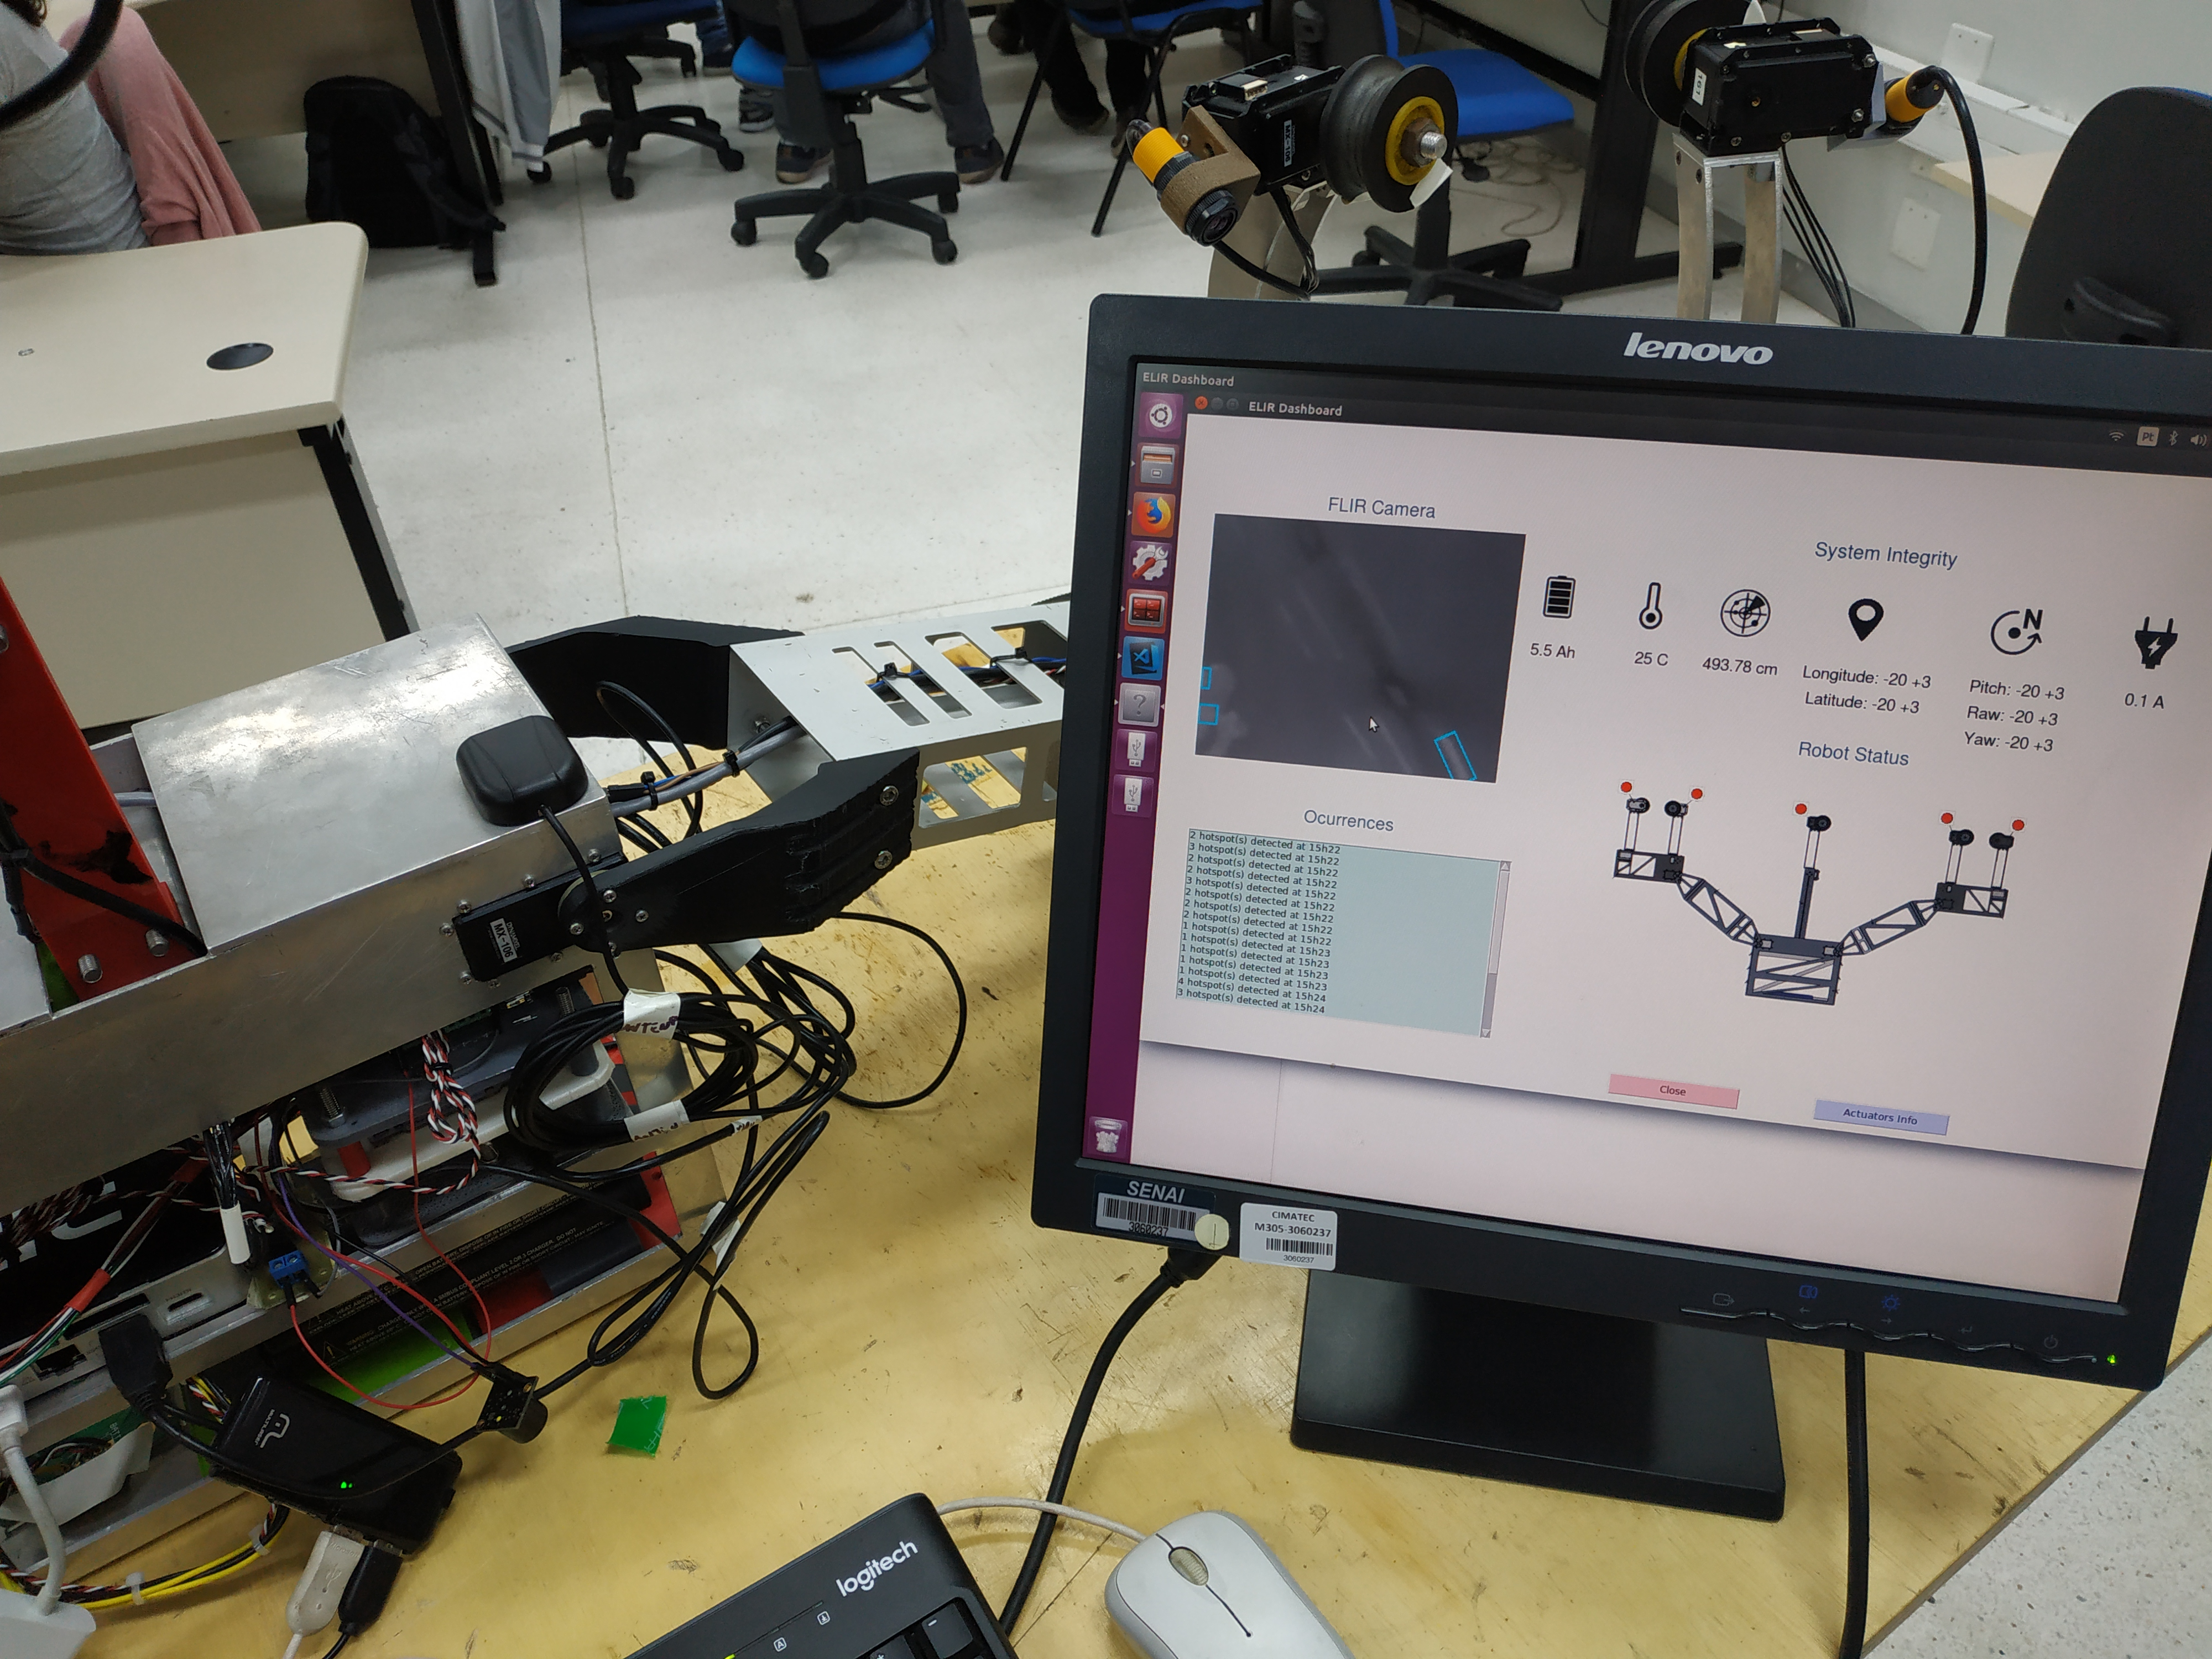
\includegraphics[width=14cm]{Figures/testintegrado.jpg}
    	\caption{Teste Integrado} \label{fig:testint}
	\end{figure}

\section{Suporte mecânico dos sensores da Percepção}

A implementação física do sistema de Percepção ocorre no processo de fixação dos sensores que a compõem no protótipo. Por tanto, foram desenvolvidos suportes utilizando impressão 3D com este fim.

Para  fixar  todos  os  sensores  e  componentes  eletrônicos  de  maneira  organizada foi desenhada uma estrutura em forma de prateleira.

 A primeira prateleira comporta os sensores do sistema de georreferenciamento que são o GPS e a IMU. A prateleira central foi projetada para a placa de interface Nucleo F401RE e por último, na terceira prateleira fica a placa de interface Phidgets.
 
As peças foram fabricadas utilizando impressão 3D e o seu desenho pode ser visto nas Figura \ref{Prateleira} e \ref{Prateleiracsensor} .

 \begin{figure}[h]
 	\centering
 	\includegraphics[width=14cm]{Figures/prateleira.png}
 	\caption{Prateleira para suporte dos componentes eletrônicos} \label{Prateleira}
 \end{figure}
 
  \begin{figure}[h]
  	\centering
  	\includegraphics[width=16cm]{Figures/prateleiracsensores.png}
  	\caption{Prateleira para suporte com sensores} \label{Prateleiracsensor}
  \end{figure}
 

Toda a parte de gerenciamento de energia do robô foi alocada em uma estrutura na parte inferior do mesmo. Esta estrutura foi projetada para comportar as baterias, a \textit{Smart Charger}, a \textit{Power Management} e a placa de interface Nucleo L432. O desenho dessa estrutura está mostrado na figura \ref{pecaaliment}.

\begin{figure}[h]
	\centering
	\includegraphics[width=14cm]{Figures/pecadebaixo.png}
	\caption{Prateleira para suporte dos componentes de alimentação} \label{pecaaliment}
\end{figure}

Todas as peças foram impressas utilizando a impressora 3D da área de robótica do SENAI CIMATEC não implicando em custos para a equipe de projeto.


 
%--------- NEW SECTION ----------------------
\section{Trabalhos futuros}
\label{sec:trabfut}
asdfadsfsdfs




